\section{Môi trường cài đặt}

SecChat được triển khai trong môi trường Docker Compose để bảo đảm kết quả chạy có thể lặp lại. Môi trường sử dụng Windows 11, Docker Desktop, Python 3, PyQt5, C/OpenSSL cho server, MySQL 8.0 cho lưu trữ, Rust/OpenMLS cho MLS bridge và TigerVNC để quan sát nhiều client đồng thời. Cấu trúc triển khai gồm một container database, một container server, một container auditor và hai container client VNC.

\begin{figure}[H]
    \centering
    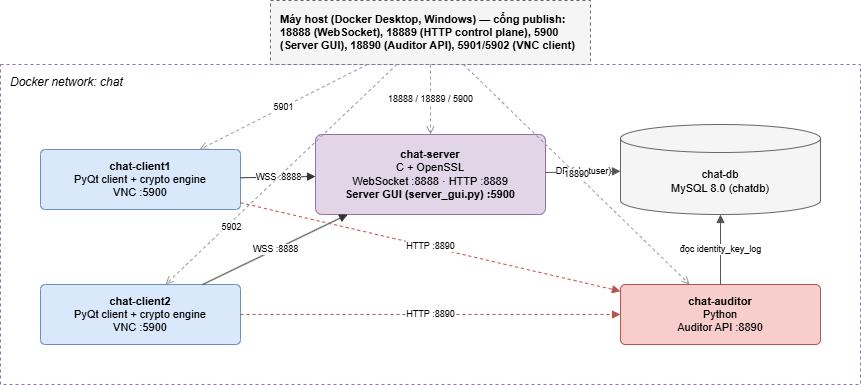
\includegraphics[width=0.95\linewidth]{Figure/DeploymentRuntime.png}
    \caption{Mô hình container khi chạy SecChat}
    \label{fig:deployment-runtime-ch3}
\end{figure}

Server WebSocket được expose tại cổng \texttt{18888}; HTTP control plane gồm \texttt{/healthz}, \texttt{/readyz} và \texttt{/metrics} được expose tại cổng \texttt{18889}. Hai client VNC dùng cổng \texttt{5901} và \texttt{5902}; server GUI dùng cổng \texttt{5900}. Trong môi trường thử nghiệm, các tài khoản \texttt{123@gmail.com}, \texttt{234@gmail.com} và \texttt{345@gmail.com} dùng mật khẩu \texttt{123456}. Các tài khoản và mật khẩu này chỉ phục vụ trình diễn cục bộ trong môi trường Docker, không được dùng trong triển khai thật. Trong môi trường thực tế, hệ thống cần bắt buộc chính sách mật khẩu mạnh và cấu hình các secret (mật khẩu cơ sở dữ liệu, khóa, chứng chỉ) riêng biệt thay vì các giá trị mặc định.

\section{Cài đặt và khởi động hệ thống}

Toàn bộ hệ thống có thể build và khởi động bằng Docker Compose. Lệnh sau tạo image, chạy migration và khởi động các service:

\begin{lstlisting}[language=bash]
docker compose up -d --build
\end{lstlisting}

Khi cần reset dữ liệu để kiểm tra lại từ trạng thái sạch, hệ thống được dừng kèm volume và khởi động lại:

\begin{lstlisting}[language=bash]
docker compose down -v
docker compose up -d --build
\end{lstlisting}

Endpoint \texttt{/readyz} được dùng để xác nhận server đã kết nối database và sẵn sàng nhận client. Khác với \texttt{/healthz}, readiness phản ánh trạng thái phụ thuộc vào MySQL nên phù hợp để kiểm tra trước khi chạy demo hoặc test.

\begin{figure}[H]
    \centering
    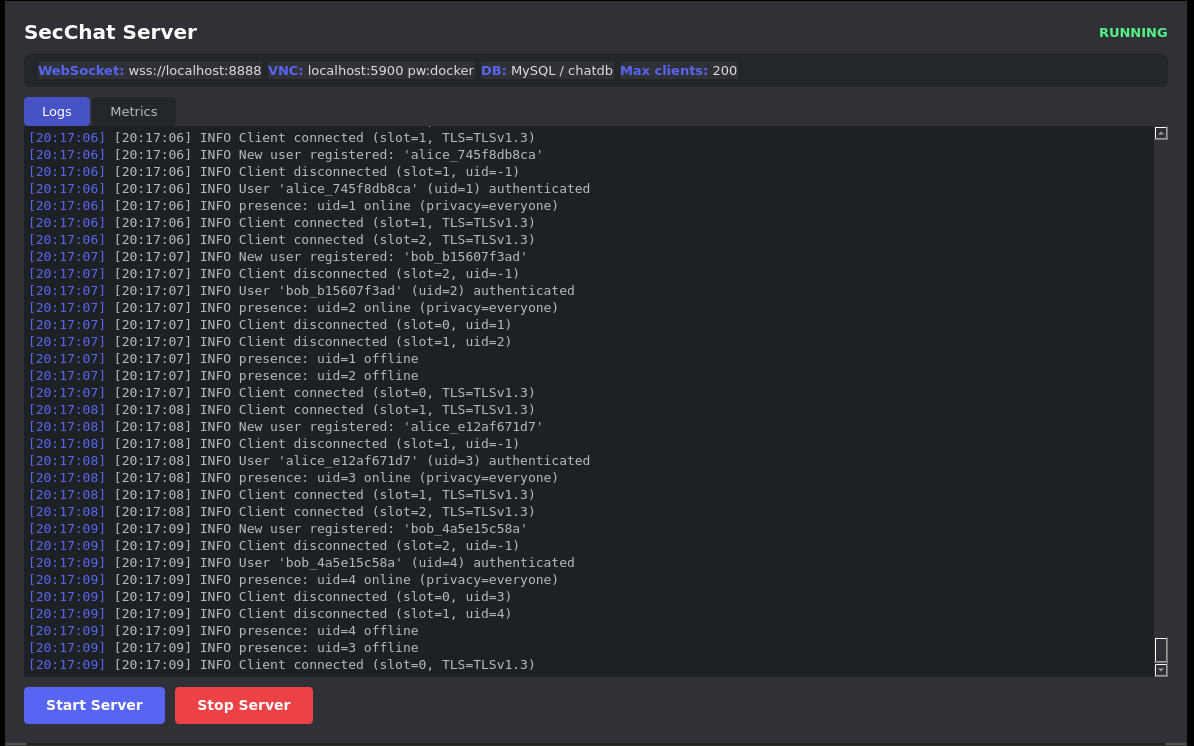
\includegraphics[width=0.95\linewidth]{Figure/ui_server_gui.png}
    \caption{Giao diện server khi hệ thống đang chạy}
    \label{fig:ui-server-gui-ch3}
\end{figure}

\section{Kết quả giao diện}

\subsection{Đăng nhập và danh sách hội thoại}

Sau khi đăng nhập, client mở local state E2EE, tải danh sách bạn bè, DM, group, request và các badge trạng thái.

\begin{figure}[H]
    \centering
    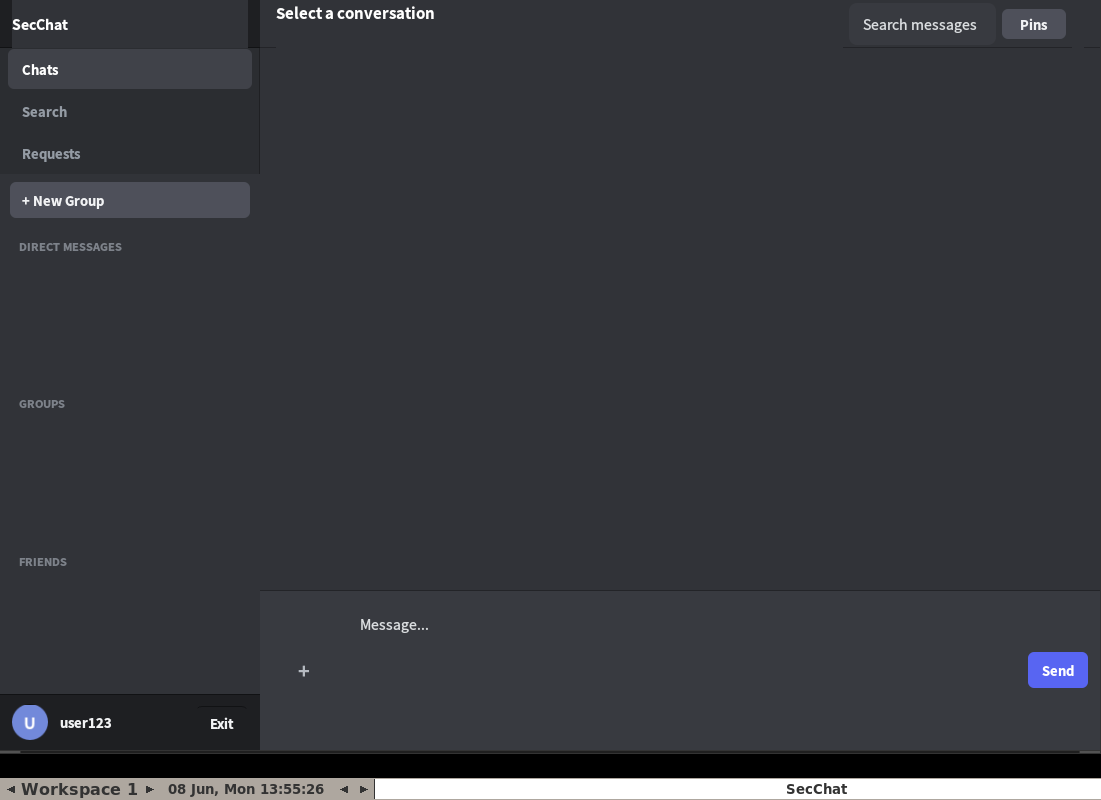
\includegraphics[width=0.95\linewidth]{Figure/ui_login_demo.png}
    \caption{Màn hình đăng nhập trong môi trường VNC}
    \label{fig:ui-login-demo}
\end{figure}

\begin{figure}[H]
    \centering
    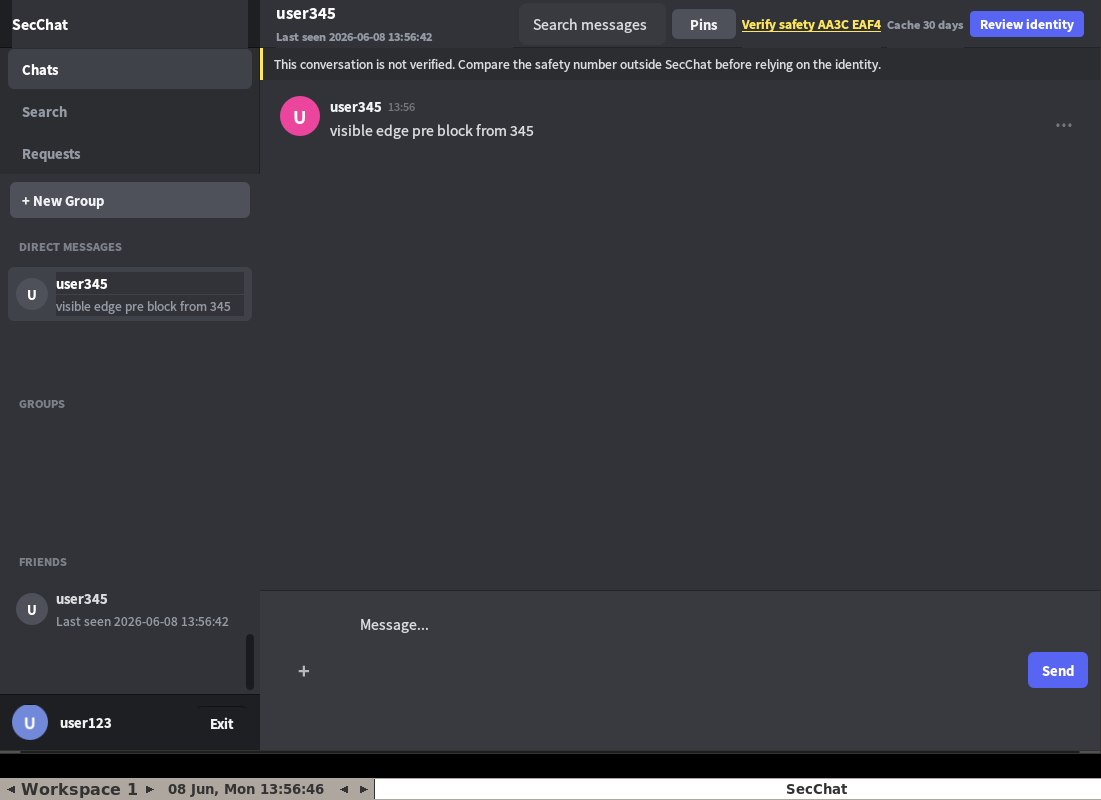
\includegraphics[width=0.95\linewidth]{Figure/ui_friend_list.png}
    \caption{Danh sách bạn bè, DM và group sau khi đăng nhập}
    \label{fig:ui-friend-list}
\end{figure}

\subsection{DM, identity và thao tác tin nhắn}

DM hiển thị header bảo mật, trạng thái review identity, message timeline và vùng nhập tin. Khi hai người dùng chưa review identity, giao diện hiển thị hướng dẫn Review identity.

\begin{figure}[H]
    \centering
    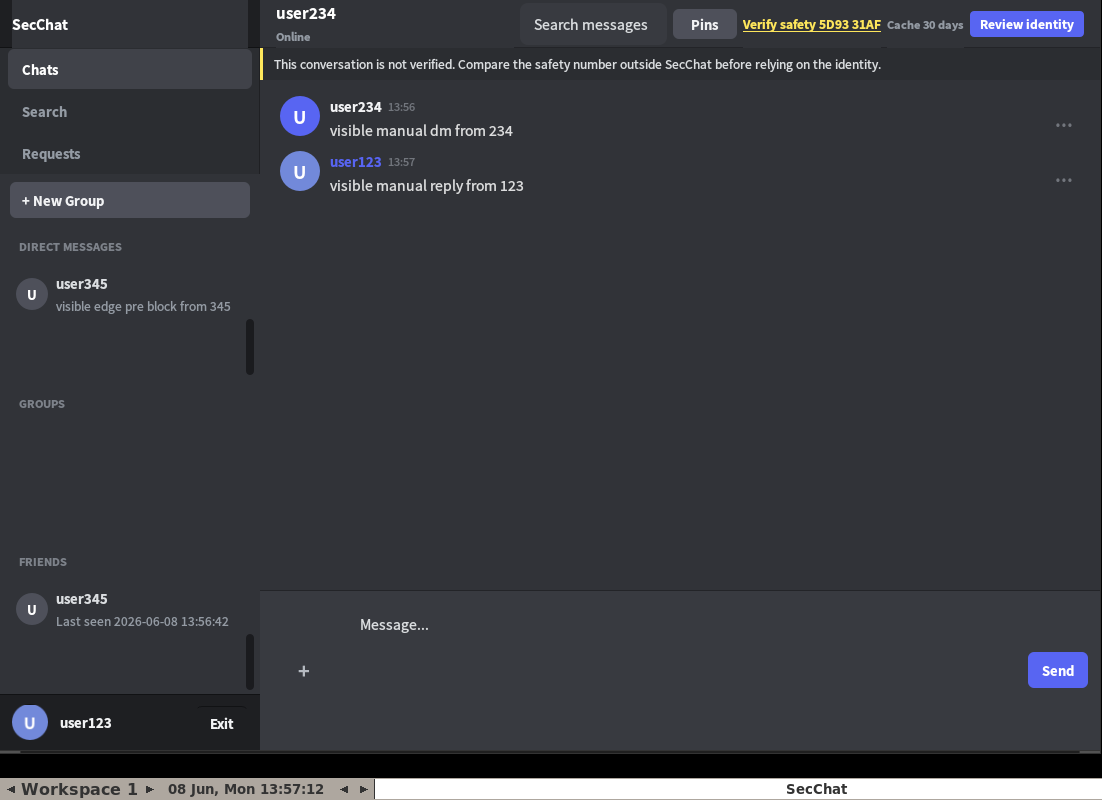
\includegraphics[width=0.95\linewidth]{Figure/ui_dm_current.png}
    \caption{Gửi nhận DM hai chiều với nội dung được giải mã ở client}
    \label{fig:ui-dm-current}
\end{figure}

\begin{figure}[H]
    \centering
    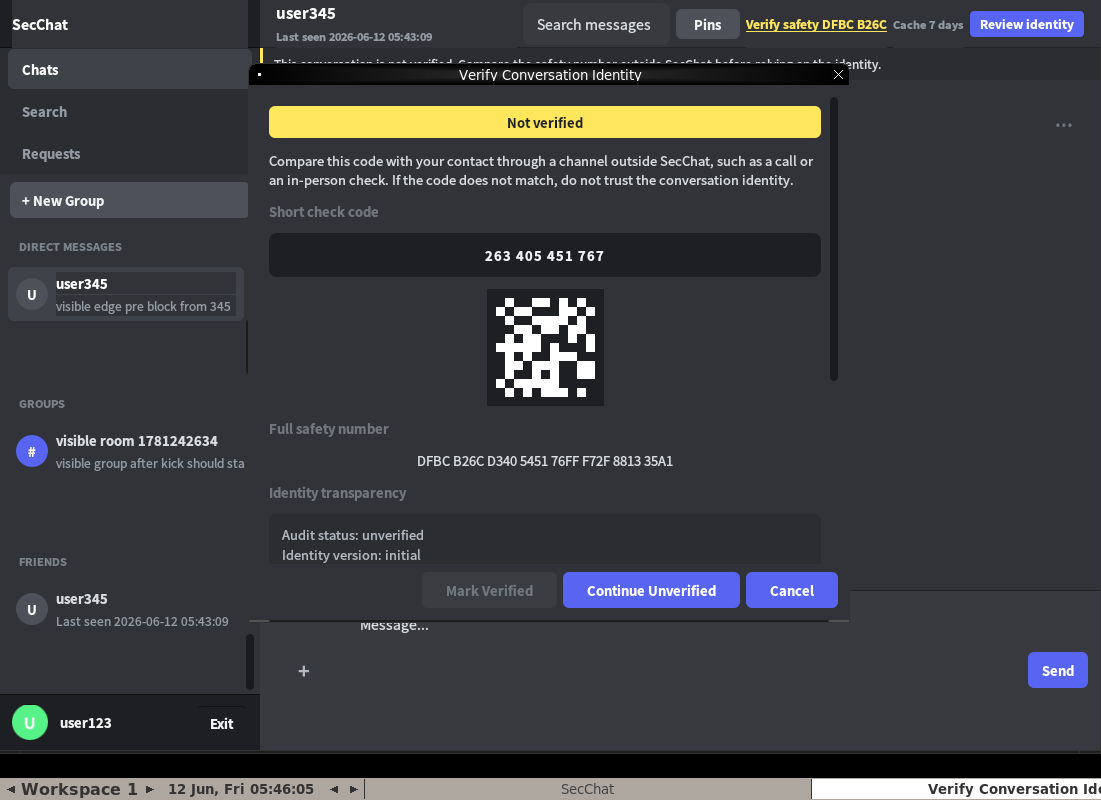
\includegraphics[width=0.95\linewidth]{Figure/ui_identity_review.png}
    \caption{Màn hình kiểm tra safety code trong DM}
    \label{fig:ui-identity-review}
\end{figure}

\begin{figure}[H]
    \centering
    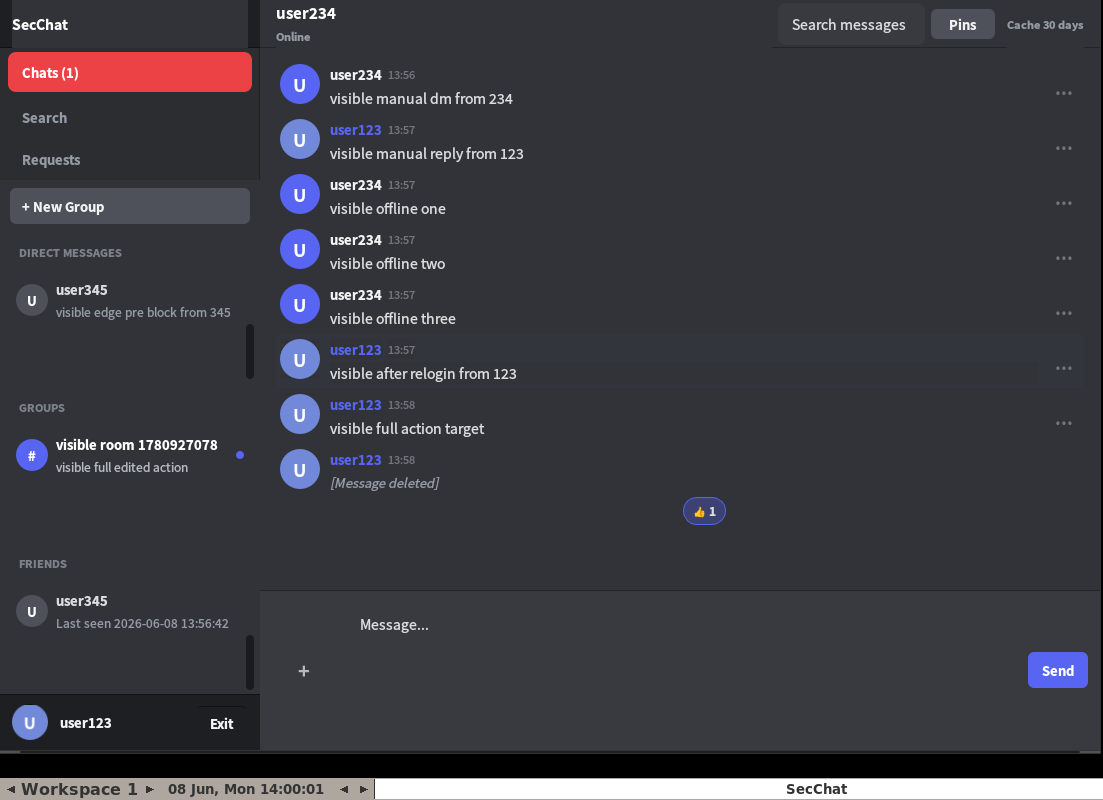
\includegraphics[width=0.95\linewidth]{Figure/ui_message_actions_current.png}
    \caption{Popover thao tác tin nhắn}
    \label{fig:ui-message-actions}
\end{figure}

\begin{figure}[H]
    \centering
    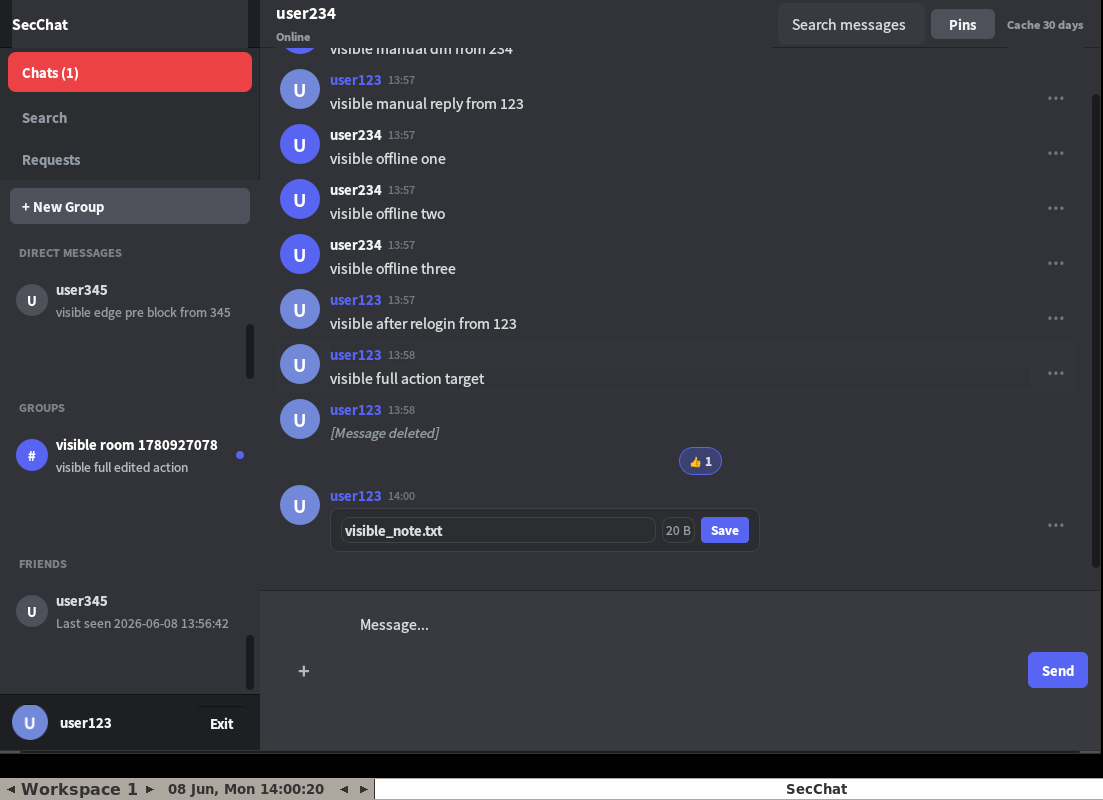
\includegraphics[width=0.95\linewidth]{Figure/ui_file_attachment_current.png}
    \caption{Gửi file trong hội thoại}
    \label{fig:ui-file-attachment}
\end{figure}

\subsection{Group chat và quản lý thành viên}

Group chat hiển thị trạng thái MLS/PQ ở header. Thay đổi member, role và thông tin group xuất hiện trong timeline như system event ổn định.

\begin{figure}[H]
    \centering
    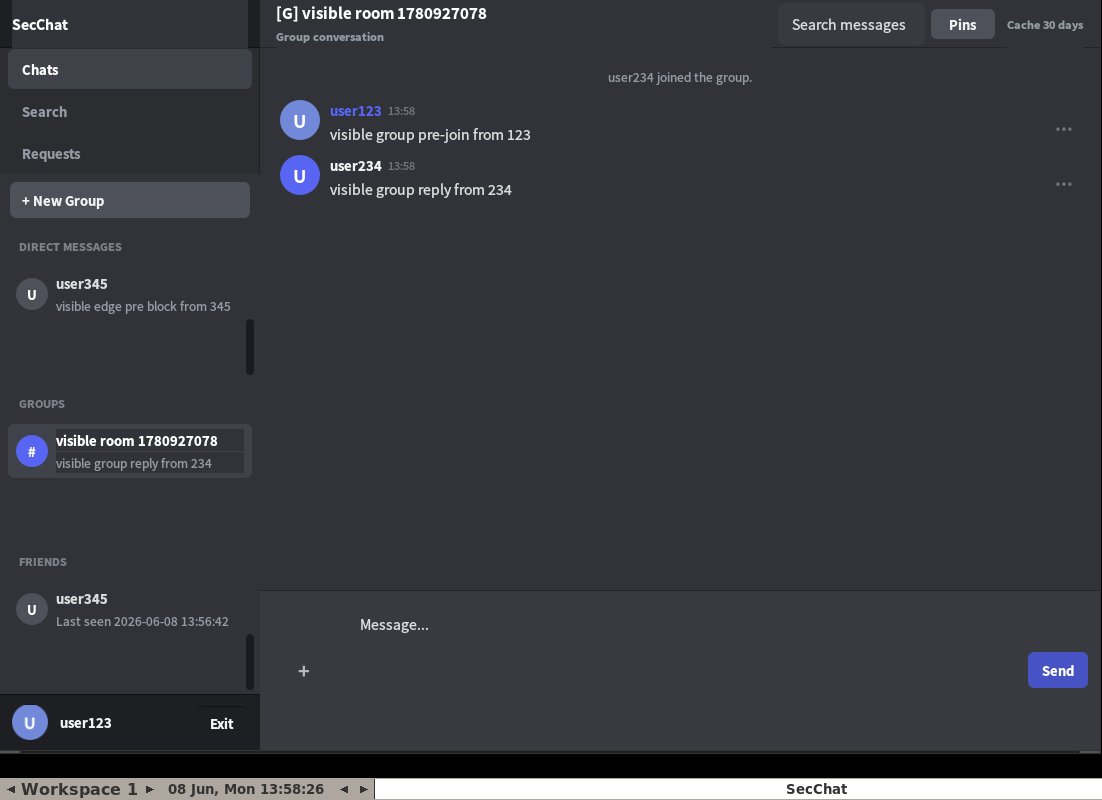
\includegraphics[width=0.95\linewidth]{Figure/ui_group_current.png}
    \caption{Màn hình group chat với trạng thái MLS/PQ}
    \label{fig:ui-group-current}
\end{figure}

\begin{figure}[H]
    \centering
    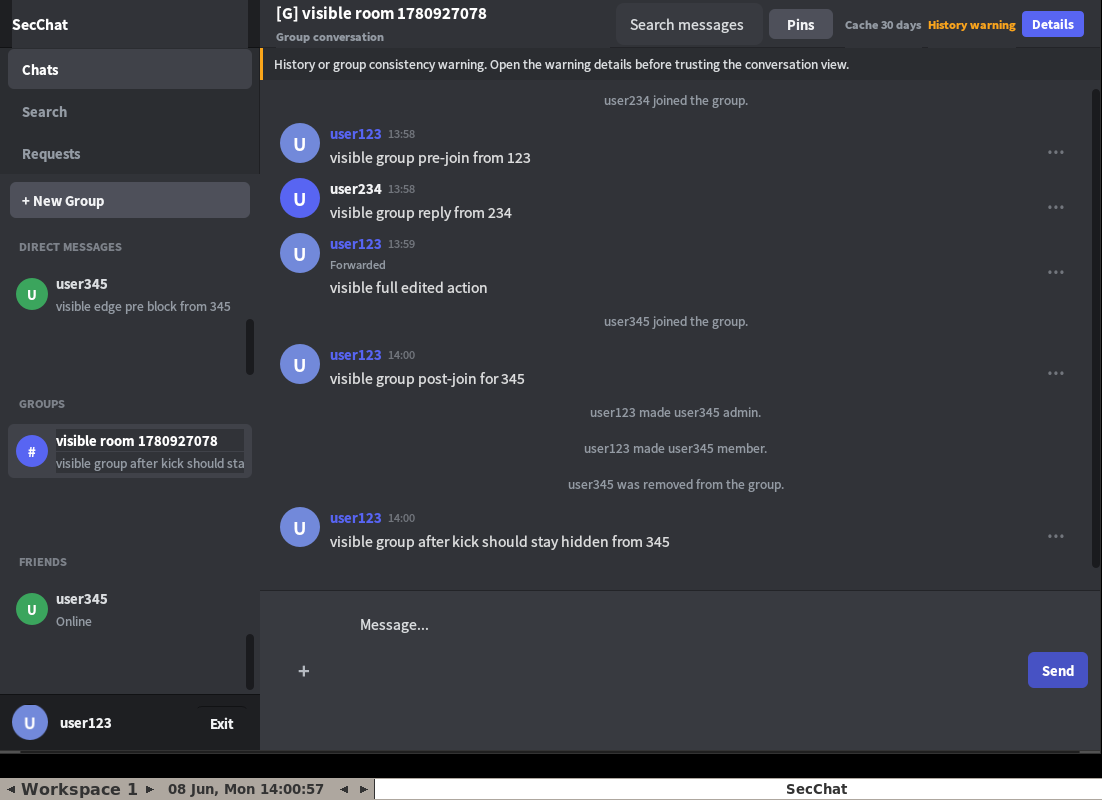
\includegraphics[width=0.95\linewidth]{Figure/ui_group_membership_current.png}
    \caption{Quản lý thành viên, role và system event trong group}
    \label{fig:ui-group-membership}
\end{figure}

\subsection{Backup, profile và trạng thái cuối}

Client cung cấp chức năng quản lý avatar, privacy, cache và backup E2EE trong profile. Backup là file do người dùng giữ, được mã hóa bằng passphrase riêng. Khi restore trên thiết bị khác, client re-wrap local state và publish public material mới mà không đưa plaintext message lên server.

\begin{figure}[H]
    \centering
    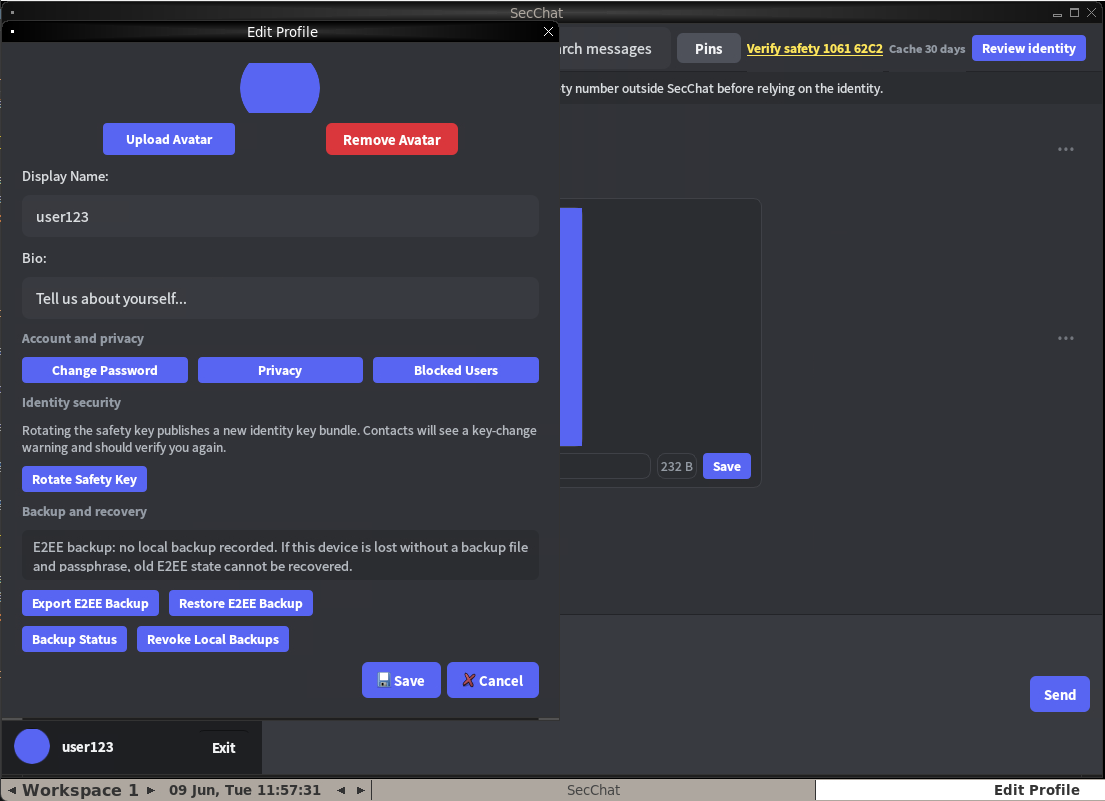
\includegraphics[width=0.95\linewidth]{Figure/3.11.png}
    \caption{Profile, privacy, avatar và backup E2EE}
    \label{fig:ui-profile-backup}
\end{figure}

\begin{figure}[H]
    \centering
    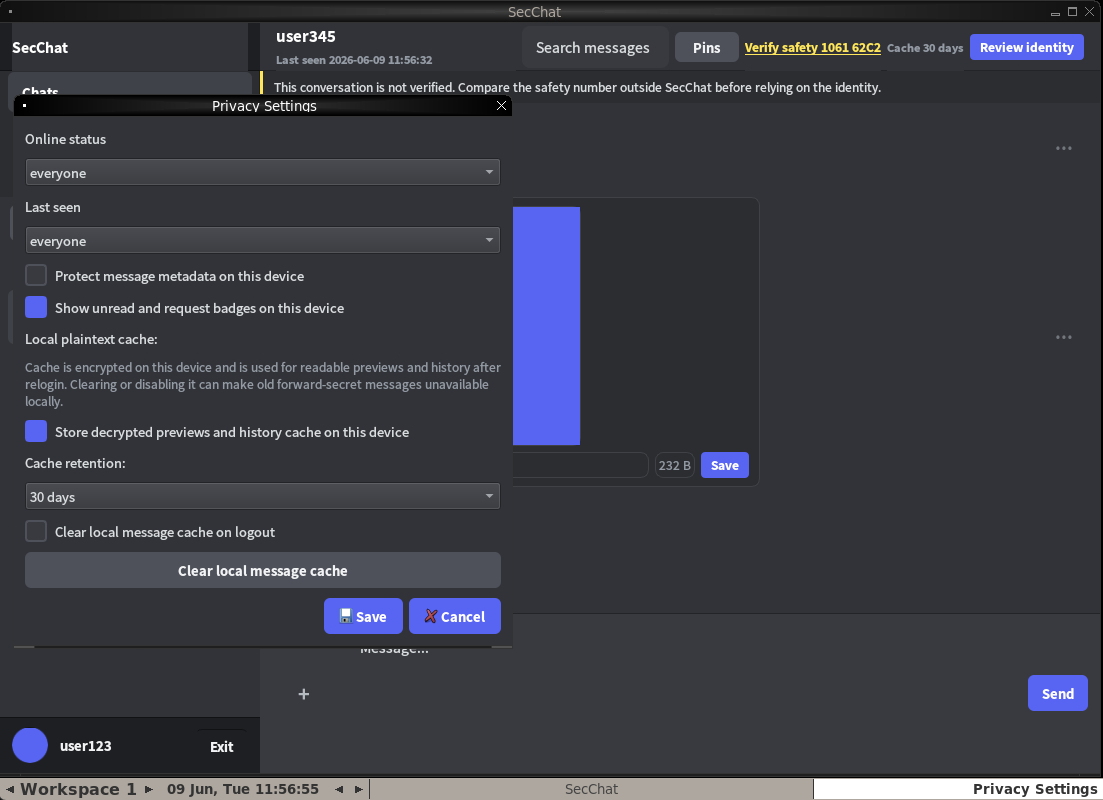
\includegraphics[width=0.95\linewidth]{Figure/3.12.png}
    \caption{Các tùy chọn privacy và cache}
    \label{fig:ui-final-core}
\end{figure}

\section{Kiểm thử chức năng}

Bộ kiểm thử tự động chạy trực tiếp trên stack Docker thật (server C, MySQL, auditor, hai client) và đối chiếu giao thức với server đang chạy. Mỗi file test chạy trong một tiến trình con riêng để một socket treo ở file này không làm hỏng file kế tiếp. Trình điều phối \texttt{tests/run\_all\_tests.py} gom 19 file thành ba nhóm và in bảng tổng kết. Kết quả: toàn bộ 19/19 file đều PASS, 0 fail (Bảng~\ref{tab:functional-test-summary}).

\begin{table}[H]
    \centering
    \small
    \begin{tabularx}{\linewidth}{|p{0.22\linewidth}|c|X|c|}
        \hline
        \textbf{Nhóm} & \textbf{Số file} & \textbf{Nội dung kiểm tra} & \textbf{KQ} \\
        \hline
        Tích hợp & 4 & Domain layer, auth/kết bạn, presence/metrics/search, chặn \& disappearing. & 4/4 \\
        \hline
        Server contract & 13 & HTTP control plane, conv prefs, privacy, multi-session, đếm metrics, giới hạn input, notification, avatar, saved messages, rate limit, identity audit, secure protocol (server), fault injection. & 13/13 \\
        \hline
        Crypto contract & 2 & Bắt tay PQXDH \& Double Ratchet, crypto session. & 2/2 \\
        \hline
        \textbf{Tổng} & \textbf{19} & & \textbf{100\%} \\
        \hline
    \end{tabularx}
    \caption{Tổng hợp kết quả kiểm thử tự động}
    \label{tab:functional-test-summary}
\end{table}

Ảnh chụp màn hình terminal của một phiên chạy trình điều phối \texttt{tests/run\_all\_tests.py} được trình bày ở Hình~\ref{fig:test-run-terminal}.

\begin{figure}[H]
    \centering
    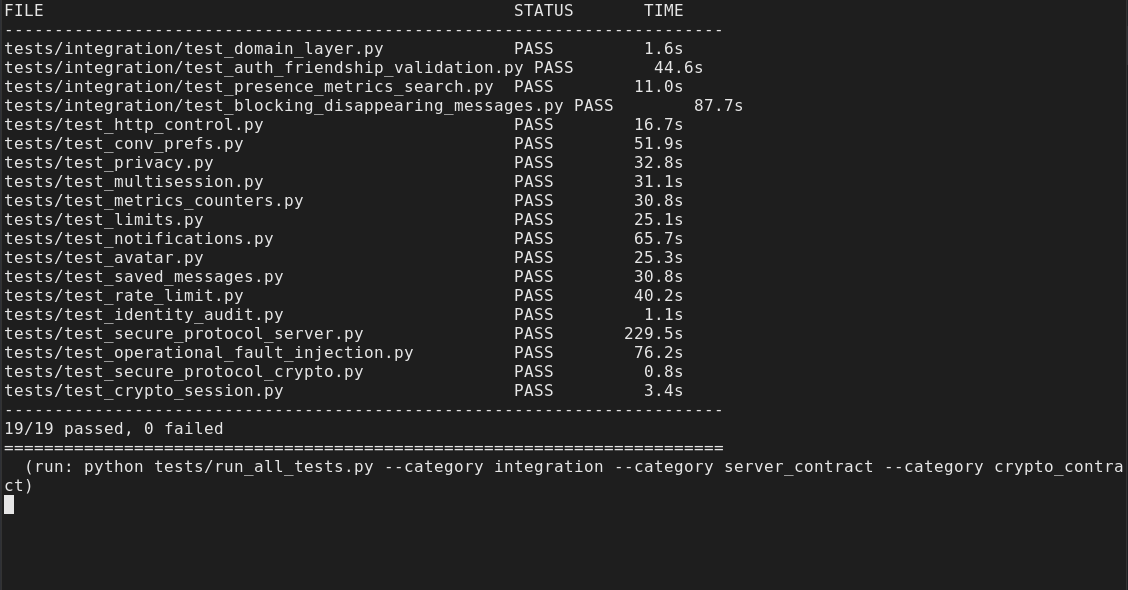
\includegraphics[width=0.95\linewidth]{Figure/ui_test_results.png}
    \caption{Kết quả chạy bộ kiểm thử tự động: 19/19 file PASS, 0 fail}
    \label{fig:test-run-terminal}
\end{figure}

Mỗi file lại gồm nhiều test-case con. Ví dụ nhóm kiểm tra tầng dữ liệu (domain) in chi tiết từng khẳng định:

\begin{figure}[H]
    \centering
    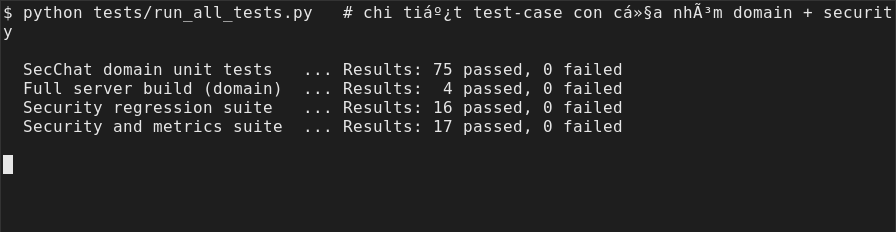
\includegraphics[width=0.78\linewidth]{Figure/ui_test_subsuites.png}
    \caption{Chi tiết test-case con: domain (75), build server (4), an toàn (16), metrics (17) đều PASS.}
    \label{fig:test-subsuites}
\end{figure}

\subsection{Kiểm thử thuộc tính an toàn}

Vì đây là hệ thống bảo mật, ngoài kiểm thử chức năng còn có các kiểm thử đối kháng: cố tình thực hiện thao tác không hợp lệ để xác nhận hệ thống từ chối đúng. Bảng~\ref{tab:security-properties} liệt kê các thuộc tính an toàn cốt lõi cùng test xác minh và kết quả.

\begin{longtable}{|p{0.30\linewidth}|p{0.34\linewidth}|p{0.12\linewidth}|c|}
\caption{Kiểm thử các thuộc tính an toàn (đối kháng)}\label{tab:security-properties}\\
\hline
\textbf{Thuộc tính} & \textbf{Cách kiểm} & \textbf{Kỳ vọng} & \textbf{KQ} \\ \hline
\endfirsthead
\hline
\textbf{Thuộc tính} & \textbf{Cách kiểm} & \textbf{Kỳ vọng} & \textbf{KQ} \\ \hline
\endhead
Server không lưu plaintext & truy vấn bảng \texttt{messages} sau hội thoại & mọi body có prefix \texttt{S3*} & Đạt \\ \hline
Body sai prefix / plaintext bị từ chối & gửi body không hợp lệ (domain validation) & server trả lỗi, không lưu & Đạt \\ \hline
Người ngoài hội thoại không thao tác được & non-member gọi \texttt{pin\_message}/history & bị từ chối & Đạt \\ \hline
Người bị chặn không gửi/không mở DM & user bị block gửi DM, mở DM mới & bị từ chối & Đạt \\ \hline
Chống brute-force đăng nhập & gửi auth sai liên tục & bị rate limit & Đạt \\ \hline
Edit không ghi đè bản gốc & chỉnh sửa tin & thêm row event trỏ về gốc & Đạt \\ \hline
Replay ciphertext cũ bị chặn & gửi lại tin có counter cũ & bị từ chối & Đạt \\ \hline
Rotate identity bị phát hiện & đổi identity rồi nhận bundle & audit báo key changed & Đạt \\ \hline
MLS validator từ chối commit sai & nạp commit/group state không hợp lệ & bị từ chối & Đạt \\ \hline
Phục hồi khi DB/server gián đoạn & tạm dừng DB/server giữa phiên & client báo lỗi rõ, không hỏng state & Đạt \\ \hline
\end{longtable}

Bằng chứng trực tiếp cho thuộc tính ``server không lưu plaintext'': sau một đợt chạy có cả nhắn tin riêng (DM) và nhắn nhóm, truy vấn thẳng bảng \texttt{messages} trong MySQL cho thấy mọi trường \texttt{body} còn lưu đều là ciphertext có prefix giao thức, không có bản rõ. Tin mở đầu mỗi cuộc DM mang prefix \texttt{S3PQI} (gói kèm transcript bắt tay PQXDH); các tin DM tiếp theo mang \texttt{S3DR} (sau khi đã vào Double Ratchet); tin nhóm mang \texttt{S3MLS} (MLS) - tất cả đều ở dạng base64:

\begin{figure}[H]
    \centering
    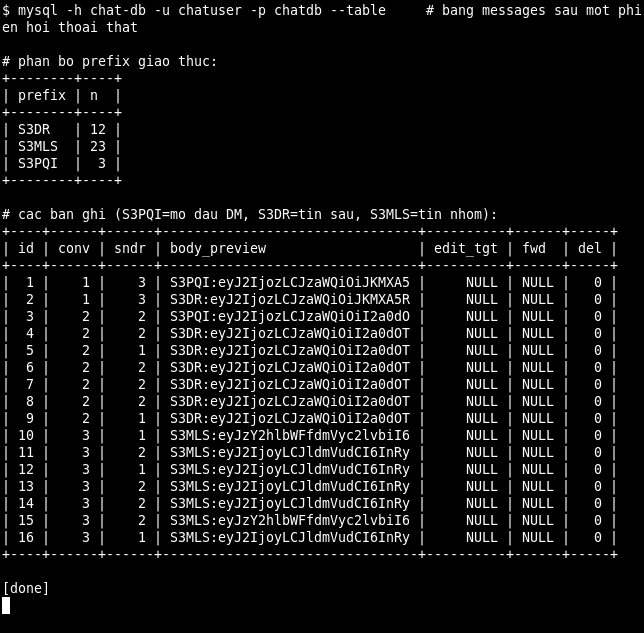
\includegraphics[width=0.82\linewidth]{Figure/ui_db_ciphertext.png}
    \caption{Bằng chứng server không lưu plaintext: truy vấn bảng \texttt{messages}; mọi \texttt{body} là ciphertext có prefix giao thức (\texttt{S3PQI} mở đầu DM, \texttt{S3DR} các tin sau, \texttt{S3MLS} tin nhóm).}
    \label{fig:db-ciphertext}
\end{figure}

\section{Kiểm toán mã nguồn server}

Server viết bằng C nên ngoài kiểm thử chức năng cần kiểm toán an toàn bộ nhớ ở tầng mã nguồn. Các lớp rủi ro cao được tập trung kiểm tra: WebSocket frame parser, JSON command parser, đường lỗi database và MLS validator. Bảng~\ref{tab:source-audit} tổng hợp phương pháp và kết quả định lượng (chạy trong container server).

Các công cụ dùng đều là công cụ kiểm thử mã C tiêu chuẩn, được giới bảo mật tin dùng: cppcheck (phân tích tĩnh), AddressSanitizer/UndefinedBehaviorSanitizer của Clang (phát hiện lỗi bộ nhớ và hành vi không xác định lúc chạy), và libFuzzer (fuzzing dẫn hướng theo độ phủ). Bảng~\ref{tab:source-audit} tổng hợp phương pháp và số liệu định lượng thu được khi chạy trong container server.

\begin{table}[H]
    \centering
    \small
    \begin{tabularx}{\linewidth}{|p{0.24\linewidth}|p{0.30\linewidth}|X|c|}
        \hline
        \textbf{Hạng mục} & \textbf{Công cụ / phương pháp} & \textbf{Số liệu thực đo} & \textbf{KQ} \\
        \hline
        Lỗi bộ nhớ / hành vi không xác định & Clang AddressSanitizer + UBSan, chạy \texttt{make asan\_test\_domain} & biên dịch sạch, chạy hết & 75/75, 0 lỗi \\
        \hline
        Phân tích tĩnh & cppcheck (error/warning/performance/ portability/style) & 36/36 file \texttt{.c} & 0 cảnh báo \\
        \hline
        WebSocket frame parser & libFuzzer \texttt{fuzz\_ws\_frame} (+ASan+UBSan) & 30.000 iter, cov 64, RSS $\approx$40\,MB & 0 crash \\
        \hline
        JSON command parser & libFuzzer \texttt{fuzz\_json\_validation} (+ASan+UBSan) & 30.000 iter, cov 700, RSS $\approx$132\,MB & 0 crash \\
        \hline
    \end{tabularx}
    \caption{Kết quả kiểm toán mã nguồn server}
    \label{tab:source-audit}
\end{table}

Output thực tế của bốn bước định lượng:

\begin{figure}[H]
    \centering
    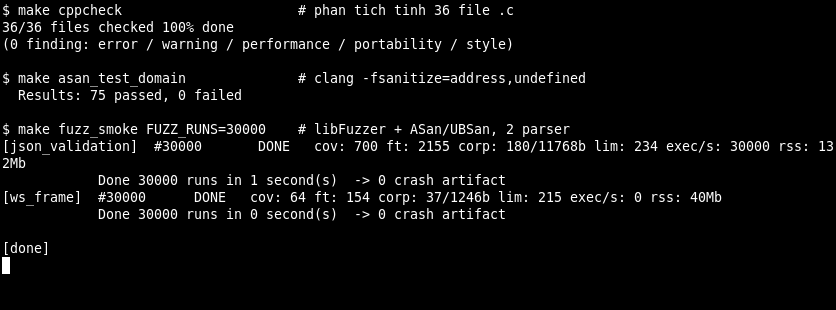
\includegraphics[width=0.86\linewidth]{Figure/ui_c_audit.png}
    \caption{Kiểm toán mã C trong container: cppcheck 36/36, ASan/UBSan 75/75, libFuzzer 30k$\times$2 0 lỗi, 0 crash.}
    \label{fig:c-audit}
\end{figure}

\subsection{Kiểm thử group MLS}

Phần MLS được hiện thực bằng OpenMLS - thư viện tham chiếu cho RFC 9420. Lệnh \texttt{secchat\_mls\_bridge selftest} chạy một vòng đầy đủ: tạo group, thêm member, phát hành Welcome, gửi application message và remove member; đồng thời kiểm tra validator chấp nhận trạng thái hợp lệ và từ chối commit giả mạo. Output JSON thực tế xác nhận ciphersuite hybrid X-Wing và các tính chất đã nêu:

\begin{figure}[H]
    \centering
    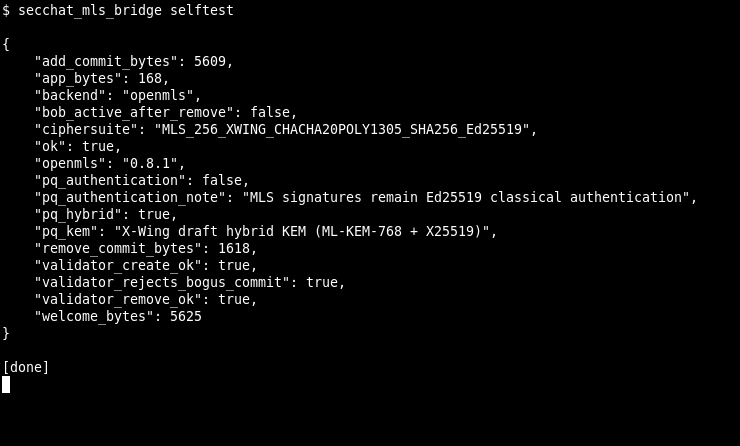
\includegraphics[width=0.74\linewidth]{Figure/ui_mls_selftest.png}
    \caption{Selftest MLS bridge (OpenMLS): ciphersuite X-Wing hybrid; validator chấp nhận state hợp lệ, từ chối commit giả mạo.}
    \label{fig:mls-selftest}
\end{figure}

\section{Đánh giá hiệu năng mật mã}\label{sec:crypto-benchmark}

Phép đo về thời gian và kích thước của các thuật toán mà SecChat sử dụng được thực hiện trong container triển khai (Linux trên Docker/WSL2, máy AMD Ryzen 5 5500U) bằng \texttt{liboqs} 0.15.0 thông qua \texttt{oqs-python} cho ML-KEM và thư viện \texttt{cryptography} cho X25519/Ed25519; mỗi giá trị là trung bình của nhiều lần lặp sau bước khởi động. Output được chụp ở Hình~\ref{fig:crypto-bench}.

\begin{table}[H]
\centering
\renewcommand{\arraystretch}{1.25}
\begin{tabularx}{\linewidth}{|X|r|r|r|r|r|r|}
\hline
\textbf{Nguyên thủy} & \textbf{\makecell{Sinh\\khóa\\(ms)}} & \textbf{\makecell{Mã hóa/\\Ký\\(ms)}} & \textbf{\makecell{Giải mã/\\Xác minh\\(ms)}} & \textbf{\makecell{Khóa\\công khai\\(B)}} & \textbf{\makecell{Khóa\\bí mật\\(B)}} & \textbf{\makecell{Bản mã/\\Chữ ký\\(B)}} \\
\hline
ML-KEM-512  & 0.020 & 0.016 & 0.016 & 800  & 1632 & 768  \\ \hline
ML-KEM-768  & 0.028 & 0.027 & 0.026 & 1184 & 2400 & 1088 \\ \hline
ML-KEM-1024 & 0.038 & 0.033 & 0.036 & 1568 & 3168 & 1568 \\ \hline
X25519 (ECDH)   & 0.041 & 0.031 & --   & 32 & 32 & 32 \\ \hline
Ed25519 (chữ ký) & 0.034 & 0.035 & 0.106 & 32 & 32 & 64 \\ \hline
\end{tabularx}
\caption{Hiệu năng các nguyên thủy mật mã của SecChat (đo trong container Linux). Với KEM, cột ``Mã hóa/Ký'' là Encaps và ``Giải mã/Xác minh'' là Decaps; với X25519 là phép trao đổi khóa.}
\label{tab:crypto-benchmark}
\end{table}

\begin{figure}[H]
    \centering
    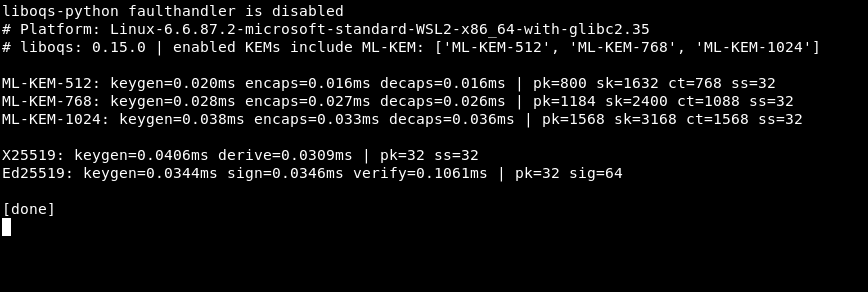
\includegraphics[width=0.92\linewidth]{Figure/ui_crypto_bench.png}
    \caption{Output của phép đo hiệu năng mật mã.}
    \label{fig:crypto-bench}
\end{figure}

Kết quả cho thấy mọi thao tác ML-KEM trong môi trường này đều ở mức vài chục micro giây (dưới một phần nghìn giây), nên việc thêm KEM hậu lượng tử vào bắt tay gần như không gây độ trễ cảm nhận được cho người dùng. Cần lưu ý các số đo X25519/Ed25519 đi qua lớp bao bọc của thư viện \texttt{cryptography} (OpenSSL) nên có thêm chi phí tạo đối tượng, vì vậy thời gian sinh khóa giữa hai họ thuật toán không hoàn toàn so sánh trực tiếp được; điểm quan trọng là tất cả đều ở mức micro giây. Chi phí thực sự nằm ở kích thước: khóa công khai và bản mã ML-KEM vào khoảng 0,8-1,6 KB, lớn hơn nhiều so với 32 byte của X25519, nhưng vẫn nhỏ so với một tin nhắn hay tệp đính kèm thông thường và hoàn toàn chấp nhận được với ứng dụng desktop. Vì SecChat dùng cấu trúc hybrid (X25519 cùng ML-KEM cho DM, và X-Wing = X25519 + ML-KEM-768 cho nhóm), tổng chi phí chỉ là phép cộng của hai cột tương ứng, đổi lại là khả năng kháng lượng tử cho khâu thiết lập khóa.


\section{Quan sát vận hành}

Để minh họa việc quan sát vận hành trực tiếp, sinh một lượng traffic ở mức bình thường rồi giữ các kết nối mở trong lúc chụp màn hình. Kịch bản tải gồm 5 client đăng ký và đăng nhập; mỗi client mở một kết nối khi đăng ký và một kết nối cho phiên làm việc, nên tổng cộng có 10 lượt kết nối được chấp nhận nhưng tối đa chỉ 6 kết nối tồn tại đồng thời. Năm client này tạo 5 quan hệ bạn bè, mở một cuộc DM hai chiều giữa hai người (mỗi bên gửi 5 tin) kèm một lượt sửa, một lượt xóa và một lượt thả cảm xúc, thêm một cuộc DM một chiều 5 tin, lập một nhóm MLS gồm 3 thành viên, rồi đọc inbox và tìm kiếm người dùng (sinh truy vấn cơ sở dữ liệu). Sau khi sinh xong, 5 kết nối được giữ mở để dashboard hiển thị đồng thời cả \emph{active connections} lẫn các bộ đếm tích lũy. Tab \emph{Metrics} của server GUI tự cập nhật mỗi 2 giây bằng cách đọc \texttt{/metrics}; các bộ đếm là tích lũy kể từ khi server khởi động và phiên đo này bắt đầu từ trạng thái đếm bằng 0. Hình~\ref{fig:ui-server-metrics-ch3} là ảnh chụp dashboard, còn Bảng~\ref{tab:ops-metrics} là số liệu \texttt{/metrics} đọc đúng thời điểm chụp.

\begin{table}[H]
    \centering
    \small
    \begin{tabular}{|p{0.50\linewidth}|p{0.38\linewidth}|}
        \hline
        \textbf{Chỉ số (phiên theo dõi)} & \textbf{Giá trị thực đo} \\
        \hline
        Phiên xác thực xử lý & 5 (ok 5 / fail 0 / rate-limited 0) \\
        \hline
        Tài khoản đăng ký & 5 \\
        \hline
        Message gửi / sửa / xóa & 16 / 1 / 1 \\
        \hline
        Tìm kiếm người dùng / bị giới hạn & 3 / 0 \\
        \hline
        Nhóm tạo / reaction & 1 / 1 \\
        \hline
        Kết nối chấp nhận / đỉnh đồng thời / đang mở & 10 / 6 / 5 \\
        \hline
        WebSocket frame nhận / gửi & 58 / 90 \\
        \hline
        Truy vấn cơ sở dữ liệu / lỗi & 41 / \textbf{0} \\
        \hline
        Độ trễ TB auth / gửi tin / DB & 218\,ms / 26\,ms / 11\,ms \\
        \hline
    \end{tabular}
    \caption{Số liệu /metrics màn hình quan sát}
    \label{tab:ops-metrics}
\end{table}

\begin{figure}[H]
    \centering
    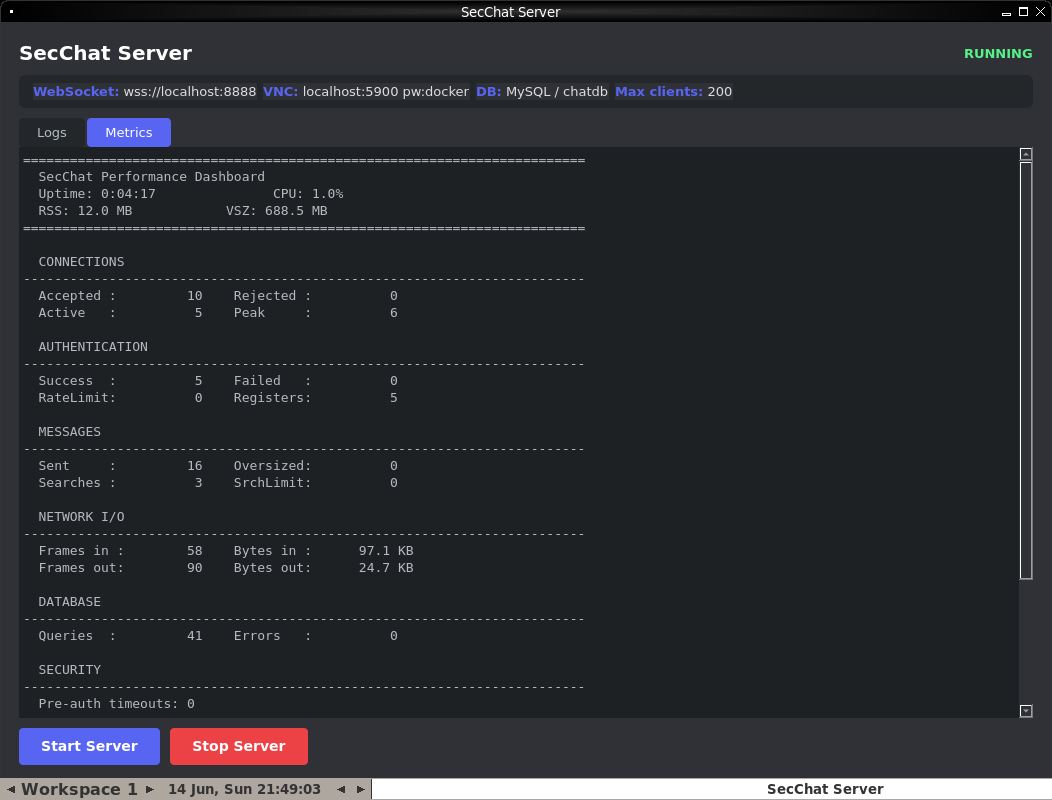
\includegraphics[width=0.95\linewidth]{Figure/ui_server_metrics.png}
    \caption{Ảnh GUI metric của server.}
    \label{fig:ui-server-metrics-ch3}
\end{figure}

Tổng hợp lại, các yêu cầu chính của sản phẩm đã được kiểm chứng: server không lưu plaintext message, DM dùng bắt tay hậu lượng tử và Double Ratchet, group dùng MLS X-Wing hybrid, server validate public MLS state trước khi thay đổi membership, timeline group giữ đúng thứ tự system event, unread state ổn định theo message id và restore E2EE hoạt động trong kịch bản nhiều thiết bị.


\section{Đánh giá bảo mật}

\subsection{Nội dung tin nhắn}

DM dùng bắt tay PQXDH-style để thiết lập secret ban đầu, sau đó dùng Double Ratchet cho từng message. Group dùng MLS theo RFC 9420 qua OpenMLS cho KeyPackage, Welcome, Commit, GroupInfo và application message. Ciphersuite group là X-Wing hybrid:
\begin{center}
    \small\texttt{MLS\_256\_XWING\_CHACHA20POLY1305\_SHA256\_Ed25519}
\end{center}
Server chỉ lưu ciphertext và public MLS artifact đã validate, không giữ secret giải mã nội dung.

Nếu ciphertext bị sửa trực tiếp trong database hoặc trên đường truyền sau khi ra khỏi TLS, client sẽ không giải mã hợp lệ. Thay vì hiển thị dữ liệu sai, UI phải hiển thị trạng thái không thể decrypt.

\subsection{Kháng lượng tử}

SecChat dùng ML-KEM trong bước thỏa thuận khóa DM, và dùng X-Wing trong MLS group. Đây là mật mã hậu lượng tử chạy bằng phần mềm. Nó khác QKD, vì QKD cần thiết bị vật lý và kênh lượng tử. Trong SecChat, dữ liệu vẫn đi qua mạng TCP/TLS bình thường.

Cơ chế hybrid trộn secret từ ML-KEM với X25519 ở DM, và trộn ML-KEM-768 với X25519 trong X-Wing ở group. Ý nghĩa của hybrid là không đặt toàn bộ niềm tin vào một giả định duy nhất. Nếu máy tính lượng tử trong tương lai phá được X25519 nhưng ML-KEM vẫn an toàn, transcript cũ vẫn có lớp bảo vệ hậu lượng tử. Nếu một giả định hậu lượng tử bị yếu trong tương lai nhưng X25519 vẫn an toàn trước attacker hiện tại, phần cổ điển vẫn đóng góp bảo vệ.

Phần hậu lượng tử của SecChat tập trung vào hai khâu: thiết lập khóa và bảo mật nội dung tin nhắn. Ngược lại, việc xác thực định danh vẫn dựa trên chữ ký Ed25519. Như đã nêu ở Chương 1, Ed25519 là một lược đồ chữ ký trên đường cong elliptic, dựa trên cùng bài toán logarit rời rạc mà thuật toán Shor phá được; do đó Ed25519 không kháng lượng tử, và một máy tính lượng tử đủ mạnh trong tương lai có thể giả mạo chữ ký định danh. Đây cũng là giới hạn của chính giao thức PQXDH mà SecChat tham chiếu: PQXDH chỉ bổ sung lớp hậu lượng tử cho bí mật của khóa phiên, còn phần xác thực lẫn nhau vẫn dựa trên độ khó của logarit rời rạc cổ điển. Vì vậy, phạm vi hậu lượng tử của đồ án tập trung vào cơ chế thiết lập khóa và bảo mật nội dung tin nhắn; thành phần xác thực định danh vẫn dùng chữ ký Ed25519 cổ điển, nên xác thực hậu lượng tử đầy đủ - chẳng hạn thay Ed25519 bằng một chữ ký hậu lượng tử như ML-DSA hoặc SLH-DSA - nằm ngoài phạm vi đồ án và là hướng phát triển tiếp theo.

\subsection{Forward secrecy và post-compromise security}

DM có Double Ratchet state, nên tốt hơn thiết kế dùng một khóa hội thoại cố định. Mỗi message dùng message key được dẫn xuất riêng. Khi ratchet state tiến lên, lộ một key ở thời điểm sau không tự động làm lộ toàn bộ quá khứ.

\subsection{Xác thực danh tính}

Identity key Ed25519 ký các prekey, giúp client phát hiện prekey không khớp với identity được công bố. Safety number giúp hai người dùng so sánh identity của nhau qua kênh khác. Khi một người rotate identity, server ghi sự kiện vào \texttt{identity\_key\_log}, auditor dựng Merkle tree và ký checkpoint. Client kiểm tra inclusion proof khi nhận bundle, lưu lịch sử identity cục bộ và hiển thị trạng thái đã xác minh, cần xác minh, key changed, \texttt{audit\_mismatch} hoặc \texttt{audit\_unavailable} trong danh sách hội thoại. Các trạng thái audit có thêm mã lỗi như identity version không có trong log, identity key không khớp, proof root không khớp, checkpoint rollback, checkpoint split-view, chữ ký checkpoint sai hoặc auditor không truy cập được.

Thao tác Mark Verified ghi nhận rằng người dùng đã so sánh safety number hoặc short check code của hội thoại hiện tại qua kênh ngoài SecChat và thấy khớp. Nó không sinh khóa mới và không làm ciphertext mạnh hơn, nhưng là quyết định quan trọng để người dùng xác nhận danh tính của peer sau cảnh báo. Nếu short check code ở hai phía khác nhau, người dùng không nên mark verified vì điều đó cho thấy hai client không đang nhìn cùng một identity state. Khi identity đổi, trạng thái đã xác minh cũ không còn đủ tin cậy và UI chuyển sang cảnh báo key changed hoặc cảnh báo audit có nguyên nhân cụ thể để người dùng review lại. Nếu người dùng restore đúng identity secret trên thiết bị mới, safety identity không đổi; peer không cần thay key, nhưng vẫn có thể cần kiểm tra lại nếu UI hiển thị cảnh báo do lịch sử identity hoặc checkpoint không đủ tin cậy. Nếu người dùng không restore và chọn rotate safety key, đây là thay đổi identity thật sự và các peer phải xem như một safety number mới.

\subsection{Metadata}

E2EE không che được toàn bộ metadata. Server vẫn biết user id, conversation id, thành viên group, thời điểm gửi, kích thước tương đối của message, trạng thái online, pin, reaction, edit target và một số sự kiện privacy-sensitive nếu người dùng bật chúng. 

Client có một số biện pháp giảm metadata như tắt typing indicator, padding plaintext trước khi mã hóa, kiểm tra consistency của history và kiểm tra commit chain của group. 

Server cũng validate public MLS state để tránh membership bị mutate bởi Commit không hợp lệ, nhưng việc này không ẩn membership khỏi server. 

Những biện pháp này giúp giảm hoặc phát hiện một số rủi ro, nhưng không làm server trở thành không cần tin cậy. Khi phát hiện history, group commit hoặc transcript checkpoint không nhất quán, UI hiển thị cảnh báo kèm nút Details để người dùng xem nguyên nhân cụ thể. Ẩn metadata mạnh hơn cần các kỹ thuật khác như sealed sender, private information retrieval, mix network hoặc delay traffic. Các kỹ thuật đó nằm ngoài phạm vi của đồ án.

\subsection{Local plaintext cache}

Local plaintext cache giúp người dùng đọc lại lịch sử sau relogin, nhất là khi ratchet state không thể decrypt lại mọi message cũ từ đầu. Cache này được mã hóa bằng master key, nên không phải plaintext thô trên ổ đĩa. Tuy nhiên nó vẫn là dữ liệu nhạy cảm. Nếu thiết bị bị chiếm và attacker có được mật khẩu hoặc master key, lịch sử cache có thể bị đọc.

Hệ thống có chính sách cache rõ: người dùng có thể tắt cache toàn cục, tắt cache cho từng conversation nhạy cảm, đặt thời gian giữ cache, xóa cache thủ công và chọn xóa cache khi logout. Cache được đặt theo tài khoản trong thư mục dữ liệu của client, nên tài khoản mới trên cùng thiết bị không được thấy cache của tài khoản cũ và cũng không được xóa cache đó. Khi export backup E2EE, người dùng chọn có đưa message cache vào file backup hay không. Đây là đánh đổi hợp lý cho trải nghiệm desktop giữa sự tiện dụng và bảo vệ dữ liệu cục bộ.

\section{Đánh giá kiến trúc phần mềm}

\subsection{Client}

Client có ranh giới rõ giữa UI, network và crypto engine. Controller chính không trực tiếp giữ toàn bộ file key, ratchet state và cache; phần lớn state nhạy cảm và thao tác mã hóa outbound nằm trong crypto engine. Điều này làm kiến trúc dễ giải thích hơn: UI gửi yêu cầu, network truyền gói, crypto engine giữ khóa và mã hóa.

Một phần decrypt message nhận vào và replay history cũng nằm trong crypto session, nhưng controller UI vẫn điều phối khá nhiều nhánh xử lý live event, history, pending key và cập nhật UI. Vì vậy crypto engine là thành phần sở hữu state nhạy cảm, còn controller UI là lớp phối hợp sự kiện.

\subsection{Server}

Repository  chịu trách nhiệm SQL, services chịu trách nhiệm nghiệp vụ, infra xử lý cấu hình và metrics, transport xử lý socket và HTTP. 

Điểm cần chú ý là server viết bằng C. C cho hiệu năng tốt và kiểm soát thấp tầng, nhưng dễ gặp lỗi memory hoặc string nếu không review kỹ. Với hệ thống bảo mật, cần tiếp tục giữ quy tắc dùng prepared statement, kiểm tra độ dài input và tránh build JSON bằng buffer không đủ kích thước.

\subsection{Cơ sở dữ liệu}

Schema bao phủ nhiều nhu cầu của app: user, profile, friendship, block, conversation, member, message, reaction, pin, notification, key bundle, prekey và public MLS state. Điều này đủ cho một ứng dụng chat desktop có nhiều tính năng.

Một điểm cần quản lý là ranh giới giữa dữ liệu phục vụ giao thức chính và dữ liệu phụ trợ cho vận hành. Những bảng lưu identity, bundle, one-time prekey, notification và message metadata phải có vai trò rõ ràng để tránh nhầm lẫn giữa khóa dùng cho E2EE và metadata server cần để điều phối hệ thống.


\section{Các nguy cơ còn lại}

Hệ thống vẫn còn một số giới hạn. Thứ nhất, group protocol dùng OpenMLS theo RFC 9420 cho flow KeyPackage, Welcome, Commit và application message, với X-Wing draft hybrid ML-KEM-768 + X25519. Đây là bảo vệ hậu lượng tử cho confidentiality, không phải authentication hậu lượng tử. Do X-Wing vẫn là draft trong hệ sinh thái MLS, hệ thống cần kế hoạch migration nếu định danh ciphersuite hoặc encoding thay đổi khi chuẩn cuối cùng ổn định.

Thứ hai, metadata chưa được ẩn. Đây là vấn đề khó và cần thiết kế riêng, không thể giải quyết chỉ bằng cách mã hóa body message.

Thứ ba, local cache giúp trải nghiệm tốt hơn nhưng làm tăng lượng dữ liệu nhạy cảm trên thiết bị. Vì vậy bảo vệ thiết bị, mật khẩu mạnh và khóa màn hình vẫn rất quan trọng.

Thứ tư, hệ thống chưa có multi-device đầy đủ. Một tài khoản chủ yếu gắn với một phiên client active tại một thời điểm. Đổi thiết bị được hỗ trợ ở mức khôi phục identity, công bố bundle mới và đọc lại lịch sử từ cache hoặc backup; hệ thống chưa có danh sách thiết bị, chưa đồng bộ ratchet state liên tục và chưa có cơ chế xác minh chéo giữa các thiết bị. Có thể cải thiện bằng cách cho mỗi thiết bị thêm identity phụ, prekey riêng và cơ chế thêm thiết bị an toàn.

\section{Hướng phát triển}

\subsection{Multi-device}

Hỗ trợ multi-device thực sự sẽ nâng cao trải nghiệm người dùng, nhưng cũng làm tăng độ phức tạp của giao thức và triển khai. Một số ý tưởng có thể nghiên cứu là thiết kế flow thêm thiết bị an toàn, đồng bộ ratchet state qua MLS hoặc server relay, và xác minh chéo identity giữa các thiết bị để phát hiện xâm nhập.

\subsection{Nâng cấp bảo vệ metadata}

Bảo vệ metadata là hướng khó nhưng có giá trị. Một số ý tưởng có thể nghiên cứu là sealed sender, giảm thông tin trong inbox, gom thời điểm gửi, hoặc thiết kế relay không biết đầy đủ quan hệ người gửi-người nhận. Đây nên được xem là một đề tài riêng, vì nó phức tạp hơn nhiều so với mã hóa nội dung.

\subsection{Cải thiện UI và nền tảng}

Có thể cải thiện tìm kiếm lịch sử, preview media, kéo thả nhiều file, trạng thái gửi thất bại, retry, notification và hỗ trợ mobile. Với mobile hoặc web, cần đặc biệt cẩn thận để không làm yếu mô hình E2EE khi chuyển key và local state sang nền tảng mới.
